%------------------------------------------------------------------------------
\section{Examples} \label{sec:example}
%------------------------------------------------------------------------------
We want to estimate the effect of 401(k) participation ({\tt p401k}) on
different conditional quantiles of net financial assets ({\tt asset}).  We
use data reported by \cite{Chernozhukov2004}.  These data are from a sample of
households in 1990 Survey of Income and Program Participation (SIPP). 
For the head of household we have data on: income ({\tt income}), age ({\tt
age}), number of people in the family ({\tt familysize}), years of education
({\tt educ}), marital status ({\tt married}), whether to participate in the IRA
({\tt ira}), whether to receive pension benefit ({\tt pension}), and whether own
a home ({\tt ownhome}).

We suspect the 401(k) participation is endogenous because it may depend on
unobserved factors such as saving preference that also impacts financial assets.
Using the 401(k) eligibility ({\tt e401k}) as an instrument for the 401(k)
participation, we use {\tt ivqregress} to estimate how the {\tt p401k} affect
the entire range of {\tt asset}'s conditional distribution. One concern about
using {\tt e401k} as an instrument is that choosing to work for a company that
offers the 401(k) program is not randomly assigned. \cite{Poterba1995} suggest
that after conditioning on the income, we can take working for a company that
offers the 401(k) plan as exogenous.

The IVQR model we want to estimate is
\begin{align}
{\tt asset}_i = {\tt p401k}_i\alpha(U) +  {\bf covariates}_i'\betab(U),  
\label{eq:asset}
\end{align}
where the distribution of $U$ conditional on instrument {\tt e401k} and
covariates is assumed to be uniform between $0$ and $1$.
The covariates are the continuous variables {\tt income}, {\tt age}, {\tt
familysize}, and {\tt educ}, and the categorical variables {\tt i.married}, {\tt
i.ira}, {\tt i.pension}, and {\tt i.ownhome}. As discussed above, {\tt e401k} is
the instrument for {\tt p401k}. The coefficients $\alpha(U)$ and $\betab(U)$ are
random because they depend on the unobserved random variable $U$, which is
uniformly distributed. In practice, $U$ can be considered a ranking variable for
the asset. When $U$ is set to a fixed level $\tau$, we are estimating an IVQR
model at a specific quantile index $\tau$. For example, when $\tau = 0.5$, we
estimate how the 401(k) participation affects the median of net financial assets
conditional on other covariates.

There are two objectives in the analysis:
\begin{enumerate}

\item Estimate the conditional quantile function of the two potential outcomes,
which are the net financial asset when everyone or no one in the population
participates in the 401(k) plan, respectively. In particular, the $\tau$-th
conditional quantile of the asset when everyone participates in the 401(k) plan
is 
$$
{\tt asset}_{\text{participate in 401(k)}} = \alpha(\tau)
+ {\bf covariates}'\betab(\tau)
$$
Similarly, the $\tau$-th conditional quantile of the asset when no one
participate in the 401(k) plan is
$$
{\tt asset}_{\text{no 401(k)}} = {\bf covariates}'\betab(\tau)
$$

\item Estimate the quantile treatment effects of 401k participation on net
financial assets. By definition, the $\tau$-th quantile treatment effect is
$$
{\tt asset}_{\text{participate in 401(k)}}
-
{\tt asset}_{\text{no 401(k)}} = \alpha(\tau)
$$

Thus, the coefficient $\alpha(\tau)$ can fully summarize the quantile treatment
effect of {\tt p401k} on {\tt asset}.

\end{enumerate}

We will show four examples that use {\tt ivqregress} to estimate the quantile
treatment effect of 401(k) participation on net financial assets. 
\begin{itemize}

\item Example 1 estimates the median treatment effect of {\tt p401k} on {\tt
asset} using the inverse quantile regression estimator. We will illustrate the
use of {\ivqreg} for estimation, how to interpret the estimates, use {\tt estat
dualci} to obtain confidence interval robust to the weak instrument, and how to
use {\tt margins} to get the conditional quantile function of the potential
outcome.

\item Example 2 is similar to Example 1 except that we use the smoothed
estimating equation estimator for estimation. We compare the results between
Example 1 and 2 and explain the difference.

\item In Example 3, we use {\ivqreg} to estimate the IVQR model at a range of
quantile indexes, use {\tt estat coefplot} to visualize quantile treatment
effects, and use {\tt estat endogeffects} to test some hypotheses of particular
interest in the context of the IVQR model.

\item Finally, Example 4 takes a closer look at the optimization procedure
underhood the IQR estimator, and uses {\tt estat waldplot} to diagnose the IQR
estimator if a non-convergence issue emerges.

\end{itemize}


%------------------------------------------------------------------------------
\subsection{Example 1: IV median regression with the IQR estimator} 
%------------------------------------------------------------------------------
In this example, we use the inverse quantile regression estimator 
to estimate the effect of 401(k) participation on the conditional median of the
net financial asset. 

\begin{stlog}
. use assets2, clear
(Excerpt from Chernozhukov and Hanson (2004) Rev. of Economics and Statistics)

\end{stlog}

\begin{stlog}
. ivqregress iqr assets (i.p401k = i.e401k) income age familysize         ///
>         i.married i.ira i.pension i.ownhome educ
{\smallskip}
Initial grid
    quantile = 0.50: .........10.........20.........30
{\smallskip}
Adaptive grid
    quantile = 0.50: .........10.........20.........30
{\smallskip}
IV median regression                                   Number of obs =   9,913
Estimator: Inverse quantile regression                 Wald chi2(9)  = 1289.75
                                                       Prob > chi2   =  0.0000
{\smallskip}
\HLI{13}{\TOPT}\HLI{64}
             {\VBAR}               Robust
      assets {\VBAR} Coefficient  std. err.      z    P>|z|     [95\% conf. interval]
\HLI{13}{\PLUS}\HLI{64}
     1.p401k {\VBAR}   5313.397   573.2818     9.27   0.000     4189.786    6437.009
      income {\VBAR}   .1577512   .0124889    12.63   0.000     .1332735    .1822289
         age {\VBAR}   99.96526   8.561923    11.68   0.000      83.1842    116.7463
  familysize {\VBAR}  -197.8251   54.36773    -3.64   0.000    -304.3838   -91.26627
             {\VBAR}
     married {\VBAR}
    Married  {\VBAR}  -1359.124   227.3366    -5.98   0.000    -1804.696   -913.5528
             {\VBAR}
         ira {\VBAR}
        Yes  {\VBAR}   22629.61   1022.706    22.13   0.000     20625.15    24634.08
             {\VBAR}
     pension {\VBAR}
Receives ..  {\VBAR}  -693.8347   210.6176    -3.29   0.001    -1106.638   -281.0317
             {\VBAR}
     ownhome {\VBAR}
        Yes  {\VBAR}  -30.29657   154.7265    -0.20   0.845     -333.555    272.9618
        educ {\VBAR}  -96.43983   32.09465    -3.00   0.003    -159.3442   -33.53547
       _cons {\VBAR}  -4998.673   570.1315    -8.77   0.000     -6116.11   -3881.236
\HLI{13}{\BOTT}\HLI{64}
Endogenous: 0b.p401k 1.p401k
 Exogenous: income age familysize 0b.married 1.married 0b.ira 1.ira
            0b.pension 1.pension 0b.ownhome 1.ownhome educ 0b.e401k 1.e401k
{\smallskip}
. estimates store est_iqr

\end{stlog}

We specify {\tt iqr} to use the inverse quantile regression. The dependent
variable is {\tt asset}. The endogenous variable {\tt i.p401k} and the
instrument {\tt i.e401k} are specified in parenthesis, the other
covariates follow as a regular {\tt varlist}. 
{\ivqreg} estimate the IV median regression by default. 


The coefficient for {\tt p401k} is \$5313. It means participation in 401(k)
would increase the median of net financial asset by \$5313 conditional on other
covariates, relative to a senario where no one participates.
We store the estimation result as {\tt est\_iqr} for later use.

After {\tt ivqregress iqr}, we can also use {\tt estat dualci} to obtain the
dual confidence interval robust to weak instrument for the coefficient on the
endogenous variables. The dual confidence interval is usually wider than the
regular confidence interval, but it provides a more robust inference if the
instrument is weak. In this example, we see that dual 95\% CI is $[\$3684,
\$7305]$, which is wider than the regular 95\% CI $[\$4178, \$6449]$.

\begin{stlog}
. estat dualci
{\smallskip}
Dual confidence interval                                 Number of obs = 9,913
\HLI{13}{\TOPT}\HLI{64}
             {\VBAR}               Robust                               Dual
      assets {\VBAR} Coefficient  std. err.      z    P>|z|     [95\% conf. interval]
\HLI{13}{\PLUS}\HLI{64}
       p401k {\VBAR}
          1  {\VBAR}   5313.397   573.2818     9.27   0.000     3683.916    7304.986
\HLI{13}{\BOTT}\HLI{64}

\end{stlog}

The coefficients on each variable summarize the quantile treatment effects of
the respective variable on the net financial asset. If we want to know
the exact quantity of the conditional median for each potential outcome,
we need to use {\tt margins}. In particular, we want to know the median of
financial assets when everyone does or does not participate in 401(k)
conditional on other covariates. We specify {\tt i.p401k} right after {\tt
margins} to tell {\tt margins} to obtain median of the asset under 401(k)
participation or no participation. The option {\tt at} specifies the values of
other covariates when computing the median. In particular, the continuous
variables such as {\tt income}, {\tt age}, {\tt familysize}, {\tt educ} are
fixed at the sample mean, and people are assumed to be married, participate in
the IRA, receive pension benefits, and own a home.

\begin{stlog}
. margins i.p401k, at((mean) income age familysize educ   ///
>         married = 1 ira = 1 pension = 1 ownhome = 1)
{\smallskip}
Adjusted predictions                                     Number of obs = 9,913
Model VCE: Robust
{\smallskip}
Expression: Linear prediction, predict()
At: income     =  37208.4 (mean)
    age        = 41.05891 (mean)
    familysize = 2.865328 (mean)
    married    =        1
    ira        =        1
    pension    =        1
    ownhome    =        1
    educ       = 13.20629 (mean)
{\smallskip}
\HLI{13}{\TOPT}\HLI{64}
             {\VBAR}            Delta-method
             {\VBAR}     Margin   std. err.      z    P>|z|     [95\% conf. interval]
\HLI{13}{\PLUS}\HLI{64}
       p401k {\VBAR}
          0  {\VBAR}   23681.37   1007.612    23.50   0.000     21706.49    25656.26
          1  {\VBAR}   28994.77   1123.076    25.82   0.000     26793.58    31195.96
\HLI{13}{\BOTT}\HLI{64}

\end{stlog}

The results show that the conditional median of assets when everyone
participates in 401(k) is \$28,995. In contrast, the conditional median of
assets when no one participates in 401(k) is only \$23,681. The difference
between these two medians is \$5313, which is the quantile treatment effect of
{\tt p401k} and is the same as the coefficient's value.

%------------------------------------------------------------------------------
\subsection{Example 2: IV median regression with the SEE estimator}
%------------------------------------------------------------------------------
In this example, we use {\tt ivqregress} to estimate the IV median regression as
in Example 1 but using the smoothed estimating equation estimator. We type {\tt
smooth} after {\tt ivqregress} to use this estimator. The model specification is
the same as in Example 1. The estimation result is stored as {\tt est\_smooth}
for later use. 

\begin{stlog}
. ivqregress smooth assets (i.p401k = i.e401k) income age familysize           
>    ///
>         i.married i.ira i.pension i.ownhome educ
{\smallskip}
Fitting smoothed IV quantile regression ...
{\smallskip}
Quantile = .5
Step 1:   bandwidth =  1302.9736    GMM criterion Q(b) =  2.617e-08
Step 2:   bandwidth =  6079.6881    GMM criterion Q(b) =  2.391e-12
Step 3:   bandwidth =  1438.3068    GMM criterion Q(b) =  8.068e-13
{\smallskip}
IV median regression                                   Number of obs =   9,913
Estimator: Smoothed estimating equations               Wald chi2(9)  = 1243.05
                                                       Prob > chi2   =  0.0000
{\smallskip}
\HLI{13}{\TOPT}\HLI{64}
             {\VBAR}               Robust
      assets {\VBAR} Coefficient  std. err.      z    P>|z|     [95\% conf. interval]
\HLI{13}{\PLUS}\HLI{64}
     1.p401k {\VBAR}   5364.468   573.3728     9.36   0.000     4240.678    6488.258
      income {\VBAR}   .1679934    .013419    12.52   0.000     .1416925    .1942942
         age {\VBAR}   113.6318   9.352867    12.15   0.000     95.30052    131.9631
  familysize {\VBAR}  -228.7766   57.61072    -3.97   0.000    -341.6916   -115.8617
             {\VBAR}
     married {\VBAR}
    Married  {\VBAR}   -1362.56   238.5988    -5.71   0.000    -1830.205   -894.9153
             {\VBAR}
         ira {\VBAR}
        Yes  {\VBAR}   22402.04   1043.504    21.47   0.000     20356.81    24447.27
             {\VBAR}
     pension {\VBAR}
Receives ..  {\VBAR}   -713.996    220.476    -3.24   0.001    -1146.121   -281.8709
             {\VBAR}
     ownhome {\VBAR}
        Yes  {\VBAR}  -12.71396   161.3703    -0.08   0.937     -328.994    303.5661
        educ {\VBAR}  -102.2889   34.18527    -2.99   0.003    -169.2908   -35.28701
       _cons {\VBAR}  -5672.645   619.7049    -9.15   0.000    -6887.244   -4458.045
\HLI{13}{\BOTT}\HLI{64}
Endogenous: 0b.p401k 1.p401k
 Exogenous: income age familysize 0b.married 1.married 0b.ira 1.ira
            0b.pension 1.pension 0b.ownhome 1.ownhome educ 0b.e401k 1.e401k
{\smallskip}
. estimates store est_smooth

\end{stlog}

The interpretation of the coefficient estimates is the same as in Example 1.
For example, the coefficient for {\tt p401k} is \$5364. So participation in
401(k) would increase the median of net financial assets by \$5364 conditional
on other covariates, relative to a senario where no one participates.

Now we can compare the coefficient on {\tt p401k} between the SEE estimator and
the IQR estimator in Example 1.

\begin{stlog}
. estat dualci
{\smallskip}
Dual confidence interval                                 Number of obs = 9,913
\HLI{13}{\TOPT}\HLI{64}
             {\VBAR}               Robust                               Dual
      assets {\VBAR} Coefficient  std. err.      z    P>|z|     [95\% conf. interval]
\HLI{13}{\PLUS}\HLI{64}
       p401k {\VBAR}
          1  {\VBAR}   5419.717   580.9771     9.33   0.000     3508.301    7407.591
\HLI{13}{\BOTT}\HLI{64}

\end{stlog}

We see that the point estimate in these two estimators are similar but not the
same. It is normal to see the different results between IQR and SEE estimators
because these two estimators approximate the original exact estimating equation
in different ways. On the one hand, the IQR estimator tries to find the solution
by an exhaust grid search. The estimation result critically depends on the range
and finesse of grid points. On the other hand, the SEE estimator uses a Kernel
method to smooth the original estimating equation. Its result depends on how
well the smoothed estimating equation approximates the original equation, mainly
controlled by the bandwidth.  

Both the IQR and SEE estimators have their advantage and weakness. The IQR
estimator is numerically stable, and it allows computing the dual confidence
interval robust to weak instruments (use {\tt estat dualci}). However, the IQR
becomes computational intensive when there is more than one endogenous variable.
Thus, {\tt ivqregress iqr} allows only one endogenous variable. In contrast, the
SEE estimator can handle multiple endogenous variables within a reasonable
computation time. However, it does not allow {\tt estat dualci} for robust
inference. In practice, if there is only one endogenous variable in the model,
we recommend using both estimators, comparing the results, and using IQR
estimator as a benchmark as it can provide valid inference even the instrument
is weak.  If there is more than one endogenous variable, we can only use {\tt
ivqregress smooth}.

As in Example 1, we can use {\tt margins} to obtain the conditional quantile
function of the potential outcome.

\begin{stlog}
. margins i.p401k, at((mean) income age familysize educ   ///
>         married = 1 ira = 1 pension = 1 ownhome = 1)
{\smallskip}
Adjusted predictions                                     Number of obs = 9,913
Model VCE: Robust
{\smallskip}
Expression: Linear prediction, predict()
At: income     =  37208.4 (mean)
    age        = 41.05891 (mean)
    familysize = 2.865328 (mean)
    married    =        1
    ira        =        1
    pension    =        1
    ownhome    =        1
    educ       = 13.20629 (mean)
{\smallskip}
\HLI{13}{\TOPT}\HLI{64}
             {\VBAR}            Delta-method
             {\VBAR}     Margin   std. err.      z    P>|z|     [95\% conf. interval]
\HLI{13}{\PLUS}\HLI{64}
       p401k {\VBAR}
          0  {\VBAR}   23550.11   1026.286    22.95   0.000     21538.63     25561.6
          1  {\VBAR}   28914.58   1142.314    25.31   0.000     26675.69    31153.47
\HLI{13}{\BOTT}\HLI{64}

\end{stlog}

The results show that the conditional median of assets when everyone
participates in 401(k) is \$28,915. In contrast, the conditional median of
assets when no one participates in 401(k) is only \$23,550.


%------------------------------------------------------------------------------
\subsection{Example 3: IVQR at different quantiles}
%------------------------------------------------------------------------------
In the first two examples, we estimate the 401(k) participation ({\tt p401k})
treatment effect on the conditional median of net financial assets ({\tt
asset}).  From the policy designer's point of view, we may be more
interested in estimating the treatment effect of {\tt p401k} on other
conditional quantiles of {\tt asset}. For example, we can ask questions like 1)
how the 401(k) participation affect the lower quantile of asset 2) are the
401(k) participation unambiguously beneficial for both lower and upper
conditional quantiles of asset. In addition, we also want to know whether
the 401(k) participation is endogenous in our model. In this example, we will
show how to use {\ivqreg} to estimate the IVQR model at different quantiles and
how to use the post-estimation tools to answer the above questions.

First, we use the IQR estimator to estimate the model at different quantiles.
In particular, we specify option {\tt quantile(10(10)90)} to estimate the IVQR
model at the 10th, 20th, \ldots, 90th quantiles. 

\begin{stlog}
. ivqregress iqr assets (i.p401k = i.e401k) income age familysize         ///
>         i.married i.ira i.pension i.ownhome educ, quantile(10(10)90)
{\smallskip}
Initial grid
    quantile = 0.10: .........10.........20.........30
    quantile = 0.20: .........10.........20.........30
    quantile = 0.30: .........10.........20.........30
    quantile = 0.40: .........10.........20.........30
    quantile = 0.50: .........10.........20.........30
    quantile = 0.60: .........10.........20.........30
    quantile = 0.70: .........10.........20.........30
    quantile = 0.80: .........10.........20.........30
    quantile = 0.90: .........10.........20.........30
{\smallskip}
Adaptive grid
    quantile = 0.10: .........10.........20.........30
    quantile = 0.20: .........10.........20.........30
    quantile = 0.30: .........10.........20.........30
    quantile = 0.40: .........10.........20.........30
    quantile = 0.50: .........10.........20.........30
    quantile = 0.60: .........10.........20.........30
    quantile = 0.70: .........10.........20.........30
    quantile = 0.80: .........10.........20.........30
    quantile = 0.90: .........10.........20.........30
{\smallskip}
IV quantile regression                                 Number of obs =   9,913
Estimator: Inverse quantile regression                 Wald chi2(81) = 5121.46
                                                       Prob > chi2   =  0.0000
{\smallskip}
\HLI{13}{\TOPT}\HLI{64}
             {\VBAR}               Robust
      assets {\VBAR} Coefficient  std. err.      z    P>|z|     [95\% conf. interval]
\HLI{13}{\PLUS}\HLI{64}
q10          {\VBAR}
     1.p401k {\VBAR}    3240.08   475.6184     6.81   0.000     2307.885    4172.275
      income {\VBAR}   .0303072   .0123138     2.46   0.014     .0061725    .0544419
         age {\VBAR}   131.5908   15.13725     8.69   0.000     101.9223    161.2592
  familysize {\VBAR}  -329.2838   123.4665    -2.67   0.008    -571.2737   -87.29385
             {\VBAR}
     married {\VBAR}
    Married  {\VBAR}  -1504.648   380.0373    -3.96   0.000    -2249.508   -759.7886
             {\VBAR}
         ira {\VBAR}
        Yes  {\VBAR}    7864.15   344.2198    22.85   0.000     7189.492    8538.809
             {\VBAR}
     pension {\VBAR}
Receives ..  {\VBAR}   63.88643   326.6017     0.20   0.845    -576.2412    704.0141
             {\VBAR}
     ownhome {\VBAR}
        Yes  {\VBAR}   969.6861   300.4319     3.23   0.001     380.8503    1558.522
        educ {\VBAR}  -301.1635   52.02897    -5.79   0.000    -403.1384   -199.1885
       _cons {\VBAR}  -7455.806   1192.112    -6.25   0.000    -9792.302   -5119.311
\HLI{13}{\PLUS}\HLI{64}
q20          {\VBAR}
     1.p401k {\VBAR}   3446.347   334.4227    10.31   0.000      2790.89    4101.803
      income {\VBAR}   .0730526   .0083383     8.76   0.000     .0567097    .0893954
         age {\VBAR}   117.4232   10.09197    11.64   0.000     97.64336    137.2031
  familysize {\VBAR}   -311.518   77.31495    -4.03   0.000    -463.0525   -159.9835
             {\VBAR}
     married {\VBAR}
    Married  {\VBAR}  -1023.821   245.1418    -4.18   0.000     -1504.29   -543.3515
             {\VBAR}
         ira {\VBAR}
        Yes  {\VBAR}   8728.335   389.1614    22.43   0.000     7965.593    9491.077
             {\VBAR}
     pension {\VBAR}
Receives ..  {\VBAR}   8.450874   211.6773     0.04   0.968     -406.429    423.3307
             {\VBAR}
     ownhome {\VBAR}
        Yes  {\VBAR}    247.107   193.7332     1.28   0.202    -132.6031     626.817
        educ {\VBAR}  -198.8986   36.72851    -5.42   0.000    -270.8852   -126.9121
       _cons {\VBAR}  -6064.723   762.7341    -7.95   0.000    -7559.654   -4569.791
\HLI{13}{\PLUS}\HLI{64}
q30          {\VBAR}
     1.p401k {\VBAR}   3674.434   318.7578    11.53   0.000      3049.68    4299.188
      income {\VBAR}   .0900328   .0080609    11.17   0.000     .0742337    .1058319
         age {\VBAR}   106.4245   8.502461    12.52   0.000        89.76     123.089
  familysize {\VBAR}  -217.4507   57.05271    -3.81   0.000     -329.272   -105.6295
             {\VBAR}
     married {\VBAR}
    Married  {\VBAR}  -1021.046   209.9362    -4.86   0.000    -1432.513   -609.5787
             {\VBAR}
         ira {\VBAR}
        Yes  {\VBAR}   11974.65   566.1735    21.15   0.000     10864.98    13084.33
             {\VBAR}
     pension {\VBAR}
Receives ..  {\VBAR}  -149.6646   187.9519    -0.80   0.426    -518.0435    218.7144
             {\VBAR}
     ownhome {\VBAR}
        Yes  {\VBAR}   118.1594   157.3384     0.75   0.453    -190.2182     426.537
        educ {\VBAR}  -122.6666   32.44148    -3.78   0.000    -186.2508   -59.08249
       _cons {\VBAR}  -5631.287   617.0855    -9.13   0.000    -6840.752   -4421.821
\HLI{13}{\PLUS}\HLI{64}
q40          {\VBAR}
     1.p401k {\VBAR}   4196.127   369.6983    11.35   0.000     3471.532    4920.722
      income {\VBAR}   .1230721   .0104554    11.77   0.000     .1025799    .1435643
         age {\VBAR}   93.83839   7.963134    11.78   0.000     78.23093    109.4458
  familysize {\VBAR}  -225.3647   51.96267    -4.34   0.000    -327.2097   -123.5198
             {\VBAR}
     married {\VBAR}
    Married  {\VBAR}  -1191.624   211.8386    -5.63   0.000     -1606.82   -776.4277
             {\VBAR}
         ira {\VBAR}
        Yes  {\VBAR}   16997.44   803.6711    21.15   0.000     15422.28    18572.61
             {\VBAR}
     pension {\VBAR}
Receives ..  {\VBAR}  -511.7032   194.9456    -2.62   0.009    -893.7895   -129.6168
             {\VBAR}
     ownhome {\VBAR}
        Yes  {\VBAR}   102.3659   148.1471     0.69   0.490     -187.997    392.7288
        educ {\VBAR}  -112.4069   30.98445    -3.63   0.000    -173.1353   -51.67845
       _cons {\VBAR}  -4787.913   553.4111    -8.65   0.000    -5872.579   -3703.247
\HLI{13}{\PLUS}\HLI{64}
q50          {\VBAR}
     1.p401k {\VBAR}   5313.397   573.2818     9.27   0.000     4189.786    6437.009
      income {\VBAR}   .1577512   .0124889    12.63   0.000     .1332735    .1822289
         age {\VBAR}   99.96526   8.561923    11.68   0.000      83.1842    116.7463
  familysize {\VBAR}  -197.8251   54.36773    -3.64   0.000    -304.3838   -91.26627
             {\VBAR}
     married {\VBAR}
    Married  {\VBAR}  -1359.124   227.3366    -5.98   0.000    -1804.696   -913.5528
             {\VBAR}
         ira {\VBAR}
        Yes  {\VBAR}   22629.61   1022.706    22.13   0.000     20625.15    24634.08
             {\VBAR}
     pension {\VBAR}
Receives ..  {\VBAR}  -693.8347   210.6176    -3.29   0.001    -1106.638   -281.0317
             {\VBAR}
     ownhome {\VBAR}
        Yes  {\VBAR}  -30.29657   154.7265    -0.20   0.845     -333.555    272.9618
        educ {\VBAR}  -96.43983   32.09465    -3.00   0.003    -159.3442   -33.53547
       _cons {\VBAR}  -4998.673   570.1315    -8.77   0.000     -6116.11   -3881.236
\HLI{13}{\PLUS}\HLI{64}
q60          {\VBAR}
     1.p401k {\VBAR}   7006.205   801.4258     8.74   0.000     5435.439     8576.97
      income {\VBAR}   .2327564   .0174037    13.37   0.000     .1986458    .2668671
         age {\VBAR}   135.4321   11.38565    11.89   0.000     113.1166    157.7475
  familysize {\VBAR}  -262.5927   65.82424    -3.99   0.000    -391.6058   -133.5795
             {\VBAR}
     married {\VBAR}
    Married  {\VBAR}  -1716.762   269.9874    -6.36   0.000    -2245.927   -1187.596
             {\VBAR}
         ira {\VBAR}
        Yes  {\VBAR}   30301.55   1241.557    24.41   0.000     27868.15    32734.96
             {\VBAR}
     pension {\VBAR}
Receives ..  {\VBAR}  -988.7325   261.4987    -3.78   0.000    -1501.261   -476.2044
             {\VBAR}
     ownhome {\VBAR}
        Yes  {\VBAR}  -122.2135   193.9046    -0.63   0.529    -502.2595    257.8324
        educ {\VBAR}  -118.7153   40.43096    -2.94   0.003    -197.9585   -39.47208
       _cons {\VBAR}  -6290.287   688.2098    -9.14   0.000    -7639.154   -4941.421
\HLI{13}{\PLUS}\HLI{64}
q70          {\VBAR}
     1.p401k {\VBAR}   9093.469   1109.745     8.19   0.000     6918.408    11268.53
      income {\VBAR}   .3459585   .0226207    15.29   0.000     .3016228    .3902942
         age {\VBAR}   191.2876   16.53737    11.57   0.000      158.875    223.7003
  familysize {\VBAR}  -242.6605   86.05014    -2.82   0.005    -411.3157   -74.00534
             {\VBAR}
     married {\VBAR}
    Married  {\VBAR}  -2470.874   352.4949    -7.01   0.000    -3161.751   -1779.996
             {\VBAR}
         ira {\VBAR}
        Yes  {\VBAR}   39365.32    1608.07    24.48   0.000     36213.56    42517.08
             {\VBAR}
     pension {\VBAR}
Receives ..  {\VBAR}  -1796.514   344.5429    -5.21   0.000    -2471.806   -1121.222
             {\VBAR}
     ownhome {\VBAR}
        Yes  {\VBAR}  -4.058645   262.5795    -0.02   0.988    -518.7051    510.5878
        educ {\VBAR}  -143.4298   51.12786    -2.81   0.005    -243.6386   -43.22104
       _cons {\VBAR}  -8637.647    928.462    -9.30   0.000     -10457.4   -6817.894
\HLI{13}{\PLUS}\HLI{64}
q80          {\VBAR}
     1.p401k {\VBAR}   10699.12   1651.062     6.48   0.000     7463.098    13935.14
      income {\VBAR}   .5103271   .0293056    17.41   0.000     .4528892    .5677649
         age {\VBAR}   280.7892   24.10894    11.65   0.000     233.5366    328.0419
  familysize {\VBAR}  -400.8973   117.2019    -3.42   0.001    -630.6089   -171.1858
             {\VBAR}
     married {\VBAR}
    Married  {\VBAR}  -2902.662   480.5005    -6.04   0.000    -3844.426   -1960.899
             {\VBAR}
         ira {\VBAR}
        Yes  {\VBAR}   48875.79   2297.873    21.27   0.000     44372.04    53379.54
             {\VBAR}
     pension {\VBAR}
Receives ..  {\VBAR}  -3072.814   502.6944    -6.11   0.000    -4058.077   -2087.551
             {\VBAR}
     ownhome {\VBAR}
        Yes  {\VBAR}   235.2409   402.9808     0.58   0.559    -554.5869    1025.069
        educ {\VBAR}   -130.398   68.51364    -1.90   0.057    -264.6823    3.886266
       _cons {\VBAR}  -11871.24   1257.402    -9.44   0.000     -14335.7   -9406.775
\HLI{13}{\PLUS}\HLI{64}
q90          {\VBAR}
     1.p401k {\VBAR}   15983.42   3046.028     5.25   0.000     10013.32    21953.53
      income {\VBAR}   .8247356   .0570029    14.47   0.000      .713012    .9364593
         age {\VBAR}   485.8734   48.99224     9.92   0.000     389.8504    581.8965
  familysize {\VBAR}  -646.4962    185.913    -3.48   0.001    -1010.879   -282.1134
             {\VBAR}
     married {\VBAR}
    Married  {\VBAR}  -3265.007   753.4701    -4.33   0.000    -4741.782   -1788.233
             {\VBAR}
         ira {\VBAR}
        Yes  {\VBAR}   68543.44   4952.261    13.84   0.000     58837.18    78249.69
             {\VBAR}
     pension {\VBAR}
Receives ..  {\VBAR}  -4656.177   869.4887    -5.36   0.000    -6360.343    -2952.01
             {\VBAR}
     ownhome {\VBAR}
        Yes  {\VBAR}   400.1957   680.2776     0.59   0.556     -933.124    1733.515
        educ {\VBAR}    48.4205   106.2844     0.46   0.649    -159.8931    256.7341
       _cons {\VBAR}  -20594.85   2260.983    -9.11   0.000     -25026.3   -16163.41
\HLI{13}{\BOTT}\HLI{64}
Endogenous: 0b.p401k 1.p401k
 Exogenous: income age familysize 0b.married 1.married 0b.ira 1.ira
            0b.pension 1.pension 0b.ownhome 1.ownhome educ 0b.e401k 1.e401k
{\smallskip}

\end{stlog}

The results show the estimates for the effect of 401(k) participation on each
conditional quantile of the asset. The interpretation of the coefficient is
similar as in Example 1 except we are looking at different conditional
quantiles. For example, for the Equation {\tt q30}, the estimates for
coefficient on {\tt p401k} is \$3674, thus participation of 401(k) would
increase the 30th conditional quantile of net financial assets by \$3674. 

In addition to looking at the exact numerical estimates from the coefficient
table, we can also use {\tt estat coefplot} to visualize the trend of {\tt
p401k}'s treatment effect from the lower to upper quantile. We specify {\tt
1.p401k} after {\tt estat coefplot} to only show the coefficient plot for the
variable {\tt 1.p401k}.

\begin{stlog}
. estat coefplot 1.p401k

\end{stlog}

\begin{figure}[H]
\centering
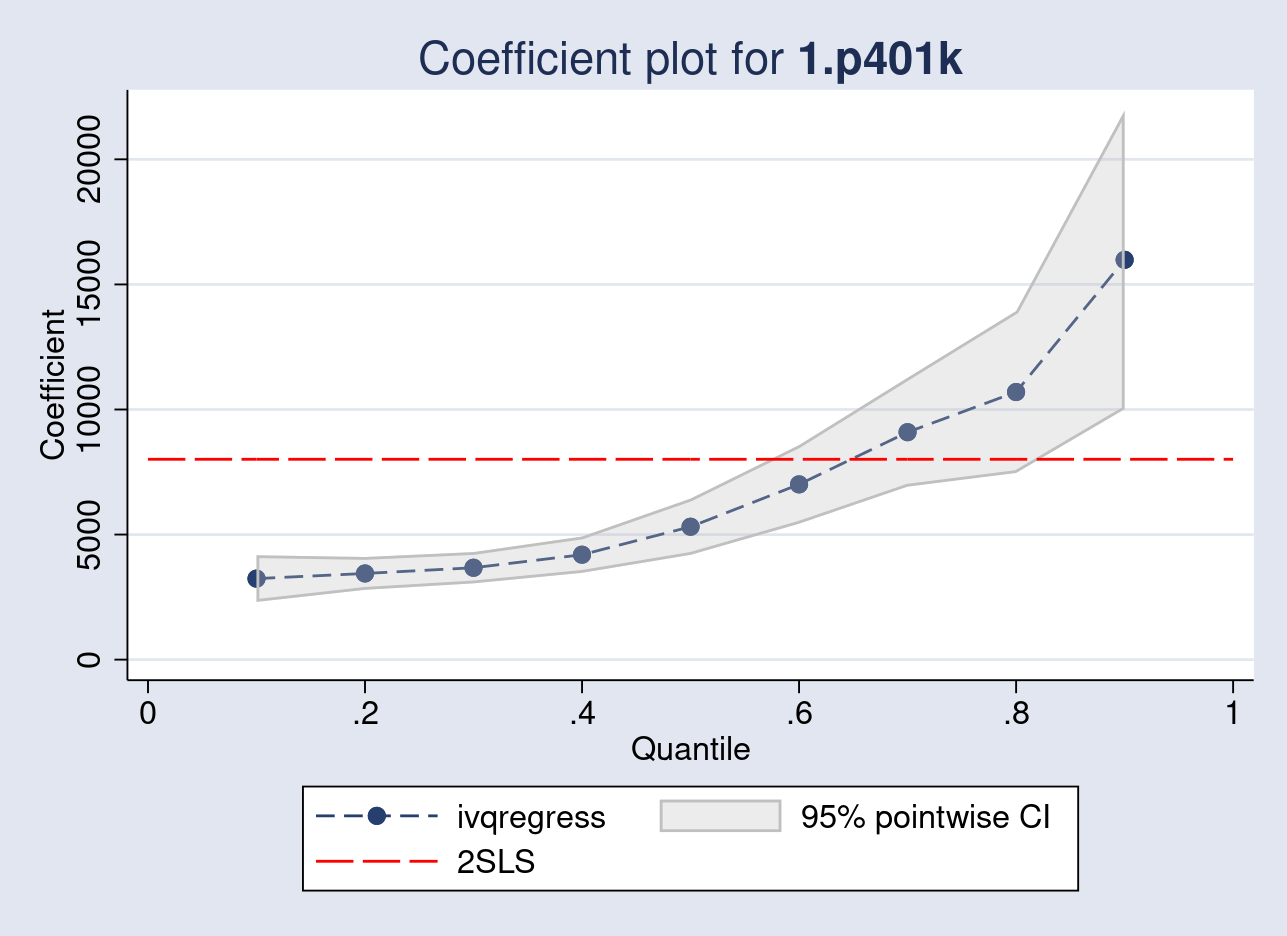
\includegraphics[scale=0.25]{eps/ex3_coefplot1}
\end{figure}

The dots in the plot show the point estimates of {\tt p401k}'s treatment effect
on different conditional quantiles of {\tt asset}, and the grey bound show the
95\% confidence interval.  We see that there is an upward trend of {\tt p401k}'s
treatment effect. At lower level quantiles such as the 10th, 20th, \ldots, 40th
quantiles, the treatment effect is relatively flat.  However, we see the
treatment effect increase significantly in the upper-level quantiles. 

{\tt estat coefplot} is a good way to visualize the treatment effect's trend. If
we want to test some hypotheses regarding the trend and the model statistically,
we can use {\tt estat endogeffects}. For example, we are interested in testing
the following hypotheses.

\begin{itemize} 

\item {\bf No effect}: The 401(k) participation does not affect net financial
asset for all the estimated quantiles; 

\item {\bf Constant effect}: The 401(k) participation's treatment effect is
constant for the different conditional quantiles of asset; 

\item {\bf Dominance}: The 401(k) participation is unambiguously beneficial for
all the estimated quantiles of asset; 

\item {\bf Exogeneity}: The 401(k) participation is exogenous.
\end{itemize}

\clearpage

\begin{stlog}
. estat endogeffects
{\smallskip}
Tests for endogenous effects           Replications = 100
\HLI{17}{\TOPT}\HLI{39}
Null hypothesis  {\VBAR}     KS statistic    95\% Critical value
\HLI{17}{\PLUS}\HLI{39}
No effect        {\VBAR}           11.271                 2.658
Constant effect  {\VBAR}            5.395                 2.650
Dominance        {\VBAR}            0.000                 2.390
Exogeneity       {\VBAR}            4.145                 2.386
\HLI{17}{\BOTT}\HLI{39}
Note: If the KS statistic < critical value, there is
      insufficient evidence to reject the null
      hypothesis.

\end{stlog}

{\tt estat endogeffects} show the Kolmogorov-Smirnov statistic and the 95\%
critical value for each hypothesis. Therefore, we reject the null hypothesis if
the test statistic is greater than the critical value. Otherwise, we can not
reject the null hypothesis.

In particular, we see that the test statistics are greater than the critical
values in testing the hypotheses of no effect, constant effect, and exogeneity.
Thus, with 95\% confidence level, we can reject these three hypotheses. In other
words, we accept the hypotheses that the 401(k) participation has some effect,
treatment is not constant across different quantiles, and 401(k) participation
is endogenous.  In contrast, we can not reject the dominance hypothesis. Thus,
we accept the hypothesis that 401(k) participation is unambiguously beneficial
for all the estimated quantiles of assets.

The test results are consistent with the result of the coefficient plot
produced by {\tt estat coefplot}, where we see that the treatment effects are
positive (dominance and no effect hypotheses) and upward trended (constant
effect hypothesis).

Finally, for reference,  we can also use the SEE estimator to estimate the
model.

\begin{stlog}
. ivqregress smooth assets (i.p401k = i.e401k) income age familysize      ///
>         i.married i.ira i.pension i.ownhome educ, quantile(10(10)90)
{\smallskip}
Fitting smoothed IV quantile regression ...
{\smallskip}
Quantile = .1
Step 1:   bandwidth =  1327.0069    GMM criterion Q(b) =  9.224e-11
Step 2:   bandwidth =  1311.3131    GMM criterion Q(b) =  1.995e-10
{\smallskip}
Quantile = .2
Step 1:   bandwidth =  1272.5204    GMM criterion Q(b) =  2.089e-10
Step 2:   bandwidth =  1237.7195    GMM criterion Q(b) =  3.075e-19
{\smallskip}
Quantile = .3
Step 1:   bandwidth =  1504.4065    GMM criterion Q(b) =  5.407e-13
Step 2:   bandwidth =  1486.4224    GMM criterion Q(b) =  1.136e-10
{\smallskip}
Quantile = .4
Step 1:   bandwidth =  1362.7753    GMM criterion Q(b) =  5.511e-17
Step 2:   bandwidth =  1362.6479    GMM criterion Q(b) =  8.561e-16
{\smallskip}
Quantile = .5
Step 1:   bandwidth =  1302.9736    GMM criterion Q(b) =  2.617e-08
Step 2:   bandwidth =  6079.6881    GMM criterion Q(b) =  2.391e-12
Step 3:   bandwidth =  1438.3068    GMM criterion Q(b) =  8.068e-13
{\smallskip}
Quantile = .6
Step 1:   bandwidth =  1533.5129    GMM criterion Q(b) =  2.679e-18
Step 2:   bandwidth =  1520.1182    GMM criterion Q(b) =  1.141e-19
{\smallskip}
Quantile = .7
Step 1:   bandwidth =  2044.8617    GMM criterion Q(b) =  1.391e-10
Step 2:   bandwidth =  1977.2482    GMM criterion Q(b) =  1.827e-11
{\smallskip}
Quantile = .8
Step 1:   bandwidth =  2503.7256    GMM criterion Q(b) =  3.623e-10
Step 2:   bandwidth =  2458.6714    GMM criterion Q(b) =  2.317e-10
{\smallskip}
Quantile = .9
Step 1:   bandwidth =  3560.2178    GMM criterion Q(b) =  4.301e-12
Step 2:   bandwidth =  3529.3557    GMM criterion Q(b) =  2.932e-10
{\smallskip}
IV quantile regression                                 Number of obs =   9,913
Estimator: Smoothed estimating equations               Wald chi2(81) = 4932.84
                                                       Prob > chi2   =  0.0000
{\smallskip}
\HLI{13}{\TOPT}\HLI{64}
             {\VBAR}               Robust
      assets {\VBAR} Coefficient  std. err.      z    P>|z|     [95\% conf. interval]
\HLI{13}{\PLUS}\HLI{64}
q10          {\VBAR}
     1.p401k {\VBAR}   3191.667   486.2193     6.56   0.000     2238.695    4144.639
      income {\VBAR}   .0318585   .0123707     2.58   0.010     .0076124    .0561046
         age {\VBAR}   128.9268   15.42632     8.36   0.000     98.69178    159.1618
  familysize {\VBAR}  -329.8374   125.4774    -2.63   0.009    -575.7687   -83.90615
             {\VBAR}
     married {\VBAR}
    Married  {\VBAR}  -1480.013   386.4611    -3.83   0.000    -2237.463   -722.5635
             {\VBAR}
         ira {\VBAR}
        Yes  {\VBAR}   7914.049   342.9506    23.08   0.000     7241.878     8586.22
             {\VBAR}
     pension {\VBAR}
Receives ..  {\VBAR}  -5.356704   334.9869    -0.02   0.987     -661.919    651.2056
             {\VBAR}
     ownhome {\VBAR}
        Yes  {\VBAR}   1043.279    308.722     3.38   0.001     438.1945    1648.363
        educ {\VBAR}  -289.8807   53.06713    -5.46   0.000    -393.8904   -185.8711
       _cons {\VBAR}  -7631.313   1214.725    -6.28   0.000    -10012.13   -5250.496
\HLI{13}{\PLUS}\HLI{64}
q20          {\VBAR}
     1.p401k {\VBAR}   3503.744   338.8383    10.34   0.000     2839.633    4167.854
      income {\VBAR}   .0737261   .0084716     8.70   0.000      .057122    .0903302
         age {\VBAR}   114.9688   10.38239    11.07   0.000     94.61965    135.3179
  familysize {\VBAR}  -277.8925   78.67289    -3.53   0.000    -432.0885   -123.6964
             {\VBAR}
     married {\VBAR}
    Married  {\VBAR}  -1160.725   253.6528    -4.58   0.000    -1657.876   -663.5752
             {\VBAR}
         ira {\VBAR}
        Yes  {\VBAR}   8799.905   388.3753    22.66   0.000     8038.703    9561.106
             {\VBAR}
     pension {\VBAR}
Receives ..  {\VBAR}  -33.33779    218.144    -0.15   0.879    -460.8921    394.2165
             {\VBAR}
     ownhome {\VBAR}
        Yes  {\VBAR}   386.2308   201.4194     1.92   0.055    -8.543996    781.0057
        educ {\VBAR}  -194.0516   37.98876    -5.11   0.000    -268.5082    -119.595
       _cons {\VBAR}  -6264.968   792.0489    -7.91   0.000    -7817.356   -4712.581
\HLI{13}{\PLUS}\HLI{64}
q30          {\VBAR}
     1.p401k {\VBAR}   3754.908   320.9631    11.70   0.000     3125.832    4383.984
      income {\VBAR}   .0939826   .0083408    11.27   0.000     .0776348    .1103303
         age {\VBAR}   103.8314   8.712147    11.92   0.000     86.75593    120.9069
  familysize {\VBAR}  -250.4947   59.95479    -4.18   0.000    -368.0039   -132.9855
             {\VBAR}
     married {\VBAR}
    Married  {\VBAR}  -1028.643   217.4311    -4.73   0.000      -1454.8   -602.4861
             {\VBAR}
         ira {\VBAR}
        Yes  {\VBAR}   12008.63   563.5555    21.31   0.000     10904.08    13113.18
             {\VBAR}
     pension {\VBAR}
Receives ..  {\VBAR}  -179.5281   192.0513    -0.93   0.350    -555.9418    196.8855
             {\VBAR}
     ownhome {\VBAR}
        Yes  {\VBAR}   195.7323    162.634     1.20   0.229    -123.0246    514.4891
        educ {\VBAR}  -134.7013    33.4085    -4.03   0.000    -200.1808   -69.22189
       _cons {\VBAR}  -5536.814   637.1917    -8.69   0.000    -6785.686   -4287.941
\HLI{13}{\PLUS}\HLI{64}
q40          {\VBAR}
     1.p401k {\VBAR}   4326.754   371.7419    11.64   0.000     3598.153    5055.354
      income {\VBAR}   .1288469   .0105877    12.17   0.000     .1080955    .1495983
         age {\VBAR}   99.89601   8.289602    12.05   0.000     83.64869    116.1433
  familysize {\VBAR}  -231.3411   53.94265    -4.29   0.000    -337.0668   -125.6155
             {\VBAR}
     married {\VBAR}
    Married  {\VBAR}  -1212.951   216.8328    -5.59   0.000    -1637.935    -787.966
             {\VBAR}
         ira {\VBAR}
        Yes  {\VBAR}   16874.38   801.2841    21.06   0.000     15303.89    18444.86
             {\VBAR}
     pension {\VBAR}
Receives ..  {\VBAR}  -493.1742   198.6221    -2.48   0.013    -882.4663   -103.8821
             {\VBAR}
     ownhome {\VBAR}
        Yes  {\VBAR}   105.4536   152.7777     0.69   0.490    -193.9852    404.8925
        educ {\VBAR}  -114.4753   32.09266    -3.57   0.000    -177.3758   -51.57484
       _cons {\VBAR}  -5216.625   581.4362    -8.97   0.000    -6356.219   -4077.031
\HLI{13}{\PLUS}\HLI{64}
q50          {\VBAR}
     1.p401k {\VBAR}   5364.468   573.3728     9.36   0.000     4240.678    6488.258
      income {\VBAR}   .1679934    .013419    12.52   0.000     .1416925    .1942942
         age {\VBAR}   113.6318   9.352867    12.15   0.000     95.30052    131.9631
  familysize {\VBAR}  -228.7766   57.61072    -3.97   0.000    -341.6916   -115.8617
             {\VBAR}
     married {\VBAR}
    Married  {\VBAR}   -1362.56   238.5988    -5.71   0.000    -1830.205   -894.9153
             {\VBAR}
         ira {\VBAR}
        Yes  {\VBAR}   22402.04   1043.504    21.47   0.000     20356.81    24447.27
             {\VBAR}
     pension {\VBAR}
Receives ..  {\VBAR}   -713.996    220.476    -3.24   0.001    -1146.121   -281.8709
             {\VBAR}
     ownhome {\VBAR}
        Yes  {\VBAR}  -12.71396   161.3703    -0.08   0.937     -328.994    303.5661
        educ {\VBAR}  -102.2889   34.18527    -2.99   0.003    -169.2908   -35.28701
       _cons {\VBAR}  -5672.645   619.7049    -9.15   0.000    -6887.244   -4458.045
\HLI{13}{\PLUS}\HLI{64}
q60          {\VBAR}
     1.p401k {\VBAR}    6964.18   799.1829     8.71   0.000     5397.811     8530.55
      income {\VBAR}   .2422267   .0180009    13.46   0.000     .2069457    .2775078
         age {\VBAR}   145.0532   11.88882    12.20   0.000     121.7515    168.3549
  familysize {\VBAR}  -271.8402   68.28584    -3.98   0.000     -405.678   -138.0024
             {\VBAR}
     married {\VBAR}
    Married  {\VBAR}   -1790.19   278.6729    -6.42   0.000    -2336.379   -1244.001
             {\VBAR}
         ira {\VBAR}
        Yes  {\VBAR}   30029.76   1251.554    23.99   0.000     27576.76    32482.76
             {\VBAR}
     pension {\VBAR}
Receives ..  {\VBAR}  -1063.919   269.4261    -3.95   0.000    -1591.984   -535.8533
             {\VBAR}
     ownhome {\VBAR}
        Yes  {\VBAR}  -79.57029   198.2018    -0.40   0.688    -468.0387    308.8981
        educ {\VBAR}  -128.4236   41.84504    -3.07   0.002    -210.4384   -46.40883
       _cons {\VBAR}  -6708.442   714.0485    -9.39   0.000    -8107.951   -5308.932
\HLI{13}{\PLUS}\HLI{64}
q70          {\VBAR}
     1.p401k {\VBAR}   9002.846   1108.915     8.12   0.000     6829.412    11176.28
      income {\VBAR}   .3555392   .0229067    15.52   0.000      .310643    .4004354
         age {\VBAR}   203.3279   17.59732    11.55   0.000     168.8378     237.818
  familysize {\VBAR}  -314.0023   89.13006    -3.52   0.000     -488.694   -139.3106
             {\VBAR}
     married {\VBAR}
    Married  {\VBAR}  -2396.634   359.7017    -6.66   0.000    -3101.636   -1691.631
             {\VBAR}
         ira {\VBAR}
        Yes  {\VBAR}   38962.04   1621.653    24.03   0.000     35783.66    42140.42
             {\VBAR}
     pension {\VBAR}
Receives ..  {\VBAR}  -1882.868   352.3168    -5.34   0.000    -2573.396    -1192.34
             {\VBAR}
     ownhome {\VBAR}
        Yes  {\VBAR}  -19.74676   271.0796    -0.07   0.942     -551.053    511.5595
        educ {\VBAR}   -163.099   52.90533    -3.08   0.002    -266.7915   -59.40646
       _cons {\VBAR}  -8753.875   954.0692    -9.18   0.000    -10623.82   -6883.934
\HLI{13}{\PLUS}\HLI{64}
q80          {\VBAR}
     1.p401k {\VBAR}   10658.02   1665.467     6.40   0.000     7393.765    13922.27
      income {\VBAR}   .5172628   .0298155    17.35   0.000     .4588255       .5757
         age {\VBAR}   293.9692   24.78395    11.86   0.000     245.3935    342.5448
  familysize {\VBAR}  -407.2737   119.8248    -3.40   0.001    -642.1259   -172.4214
             {\VBAR}
     married {\VBAR}
    Married  {\VBAR}   -3077.77   491.0029    -6.27   0.000    -4040.118   -2115.422
             {\VBAR}
         ira {\VBAR}
        Yes  {\VBAR}   48410.11   2296.042    21.08   0.000     43909.95    52910.27
             {\VBAR}
     pension {\VBAR}
Receives ..  {\VBAR}  -3049.023   515.0161    -5.92   0.000    -4058.436    -2039.61
             {\VBAR}
     ownhome {\VBAR}
        Yes  {\VBAR}   272.4814   412.1642     0.66   0.509    -535.3457    1080.308
        educ {\VBAR}  -131.0776   69.87187    -1.88   0.061    -268.0239    5.868784
       _cons {\VBAR}  -12294.73   1284.692    -9.57   0.000    -14812.68   -9776.781
\HLI{13}{\PLUS}\HLI{64}
q90          {\VBAR}
     1.p401k {\VBAR}   15525.23   3035.965     5.11   0.000     9574.848    21475.61
      income {\VBAR}   .8311508   .0574108    14.48   0.000     .7186277    .9436738
         age {\VBAR}   486.9876   51.61654     9.43   0.000      385.821    588.1541
  familysize {\VBAR}  -586.2617   193.5936    -3.03   0.002    -965.6983   -206.8252
             {\VBAR}
     married {\VBAR}
    Married  {\VBAR}  -3877.165   781.2296    -4.96   0.000    -5408.347   -2345.983
             {\VBAR}
         ira {\VBAR}
        Yes  {\VBAR}   67888.86   4902.106    13.85   0.000     58280.91    77496.81
             {\VBAR}
     pension {\VBAR}
Receives ..  {\VBAR}  -4829.506   898.9147    -5.37   0.000    -6591.346   -3067.665
             {\VBAR}
     ownhome {\VBAR}
        Yes  {\VBAR}   715.6272   722.8727     0.99   0.322    -701.1773    2132.432
        educ {\VBAR}    14.5293   110.8781     0.13   0.896    -202.7878    231.8464
       _cons {\VBAR}  -19953.21   2326.698    -8.58   0.000    -24513.45   -15392.96
\HLI{13}{\BOTT}\HLI{64}
Endogenous: 0b.p401k 1.p401k
 Exogenous: income age familysize 0b.married 1.married 0b.ira 1.ira
            0b.pension 1.pension 0b.ownhome 1.ownhome educ 0b.e401k 1.e401k
{\smallskip}

\end{stlog}

As seen above, after {\tt ivqregress smooth}, we can use {\tt estat coefplot} to
visualize the treatment effect and {\tt estat endogeffects} to test some
hypotheses of particular interest in the context of the IVQR model. To save
space, we will not list the result here.

%------------------------------------------------------------------------------
\subsection{Example 4: Diagnose the IQR estimator}
%------------------------------------------------------------------------------
In this example, we will take a closer look at the IQR estimator and show how to
diagnose the non-convergence issue if it happens. Let us first briefly talk
about the algorithm in the IQR estimator in the context of the 401(k) example.
Intuitively, the IQR estimator can be divided into the following steps.

\begin{enumerate}
\item Define a series of $A = \{\alpha_j\}_{j=1}^J$, where $J$ is the number of
grid points and it can be specified via option {\tt ngrid()}, and $\alpha_j$ is
a candidate solution for the coefficient on {\tt 1.p401k}.

\item For each $\alpha_j$, run the quantile regression of ${\tt asset} - {\tt
1.p401k}*\alpha_j$ on the covariates and some transformations of instruments.
Denote $\gammab_j$ as the coefficients on the instruments and $\Wb_j$ as the
Wald statistic for $\gammab_j$.

\item The IQR solution for $\alpha$ (the coefficients on {\tt 1.p401k}) is the
$\alpha_j$ such that $\gammab_j$ is closest to zero. In other words, the
solution chooses $\alpha_j$ such that the Wald statistic $\Wb_j$ is the
smallest.

\end{enumerate}

We can use {\tt estat waldplot} to visualize the above procedure. Using the
estimation result in Example 1, we first restore the result {\tt est\_iqr} and
then use {\tt estat waldplot} to draw the Wald statistics corresponding to each
grid points.

\begin{stlog}
. estimates restore est_iqr
(results est_iqr are active now)
{\smallskip}
. estat waldplot, name(a)

\end{stlog}

\begin{figure}[H]
\centering
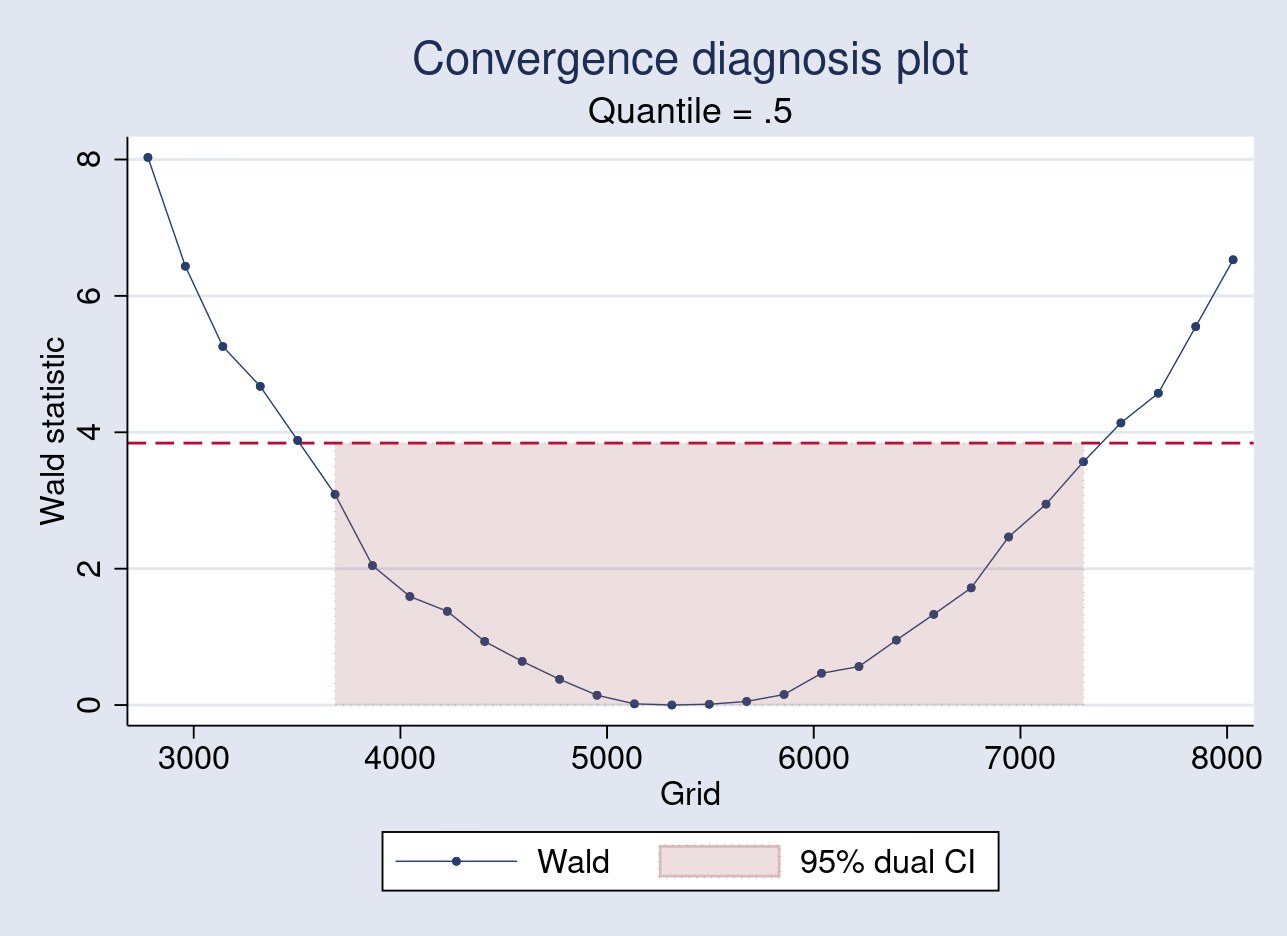
\includegraphics[scale=0.25]{eps/ex4_waldplot1}
\end{figure}

The horizontal axis shows the grid points for $\alpha$, and the vertical axis
shows the values of Wald statistics. Each dot in the plot shows the Wald
statistic corresponding to each grid point. The red dashed line is the 95\%
critical value of the Wald test. Thus, only the Wald statistics below the red
dashed line will not reject the hypothesis that $\gammab_j$ equals zero.
Respectively, the 95\% dual confidence interval is the $\alpha$'s such that the
Wald statistics are below the critical value. See Example 1 for the use of {\tt
estat dualci} to show the numerical values of the dual CI.

By default, {\tt ivqregress iqr} uses the dual CI to generate the lower and
upper bound for the grid points to make sure that the grid covers the true value
of parameter $\alpha$ with a big probability. Sometimes, we may want to
customize the bounds. For example, suppose we want to search grid points between
$3000$ and $6000$. We can use option {\tt bound()} for this purpose.

\begin{stlog}
. cap noi ivqregress iqr assets (i.p401k = i.e401k) income age familysize  ///
>         i.married i.ira i.pension i.ownhome educ, bound(3000 6000)
{\smallskip}
Initial grid
    quantile = 0.50: .........10.........20.........30
{\smallskip}
convergence not achieved
    The grid interval should be wider than the 95\% dual confidence interval.
    Try to set a wider bound using option {\bftt{bound()}}. Use {\bftt{estat waldplot}} for
    diagnosis.

\end{stlog}

We see that {\ivqreg} errors out with ``convergence not achieved". The reason is
that the specified bound is too narrow to cover the true value of the parameter
with a 95\% probability. We can use {\tt estat waldplot} to further visualize
the issue.

\begin{stlog}
. estat waldplot, name(b)

\end{stlog}

\begin{figure}[H]
\centering
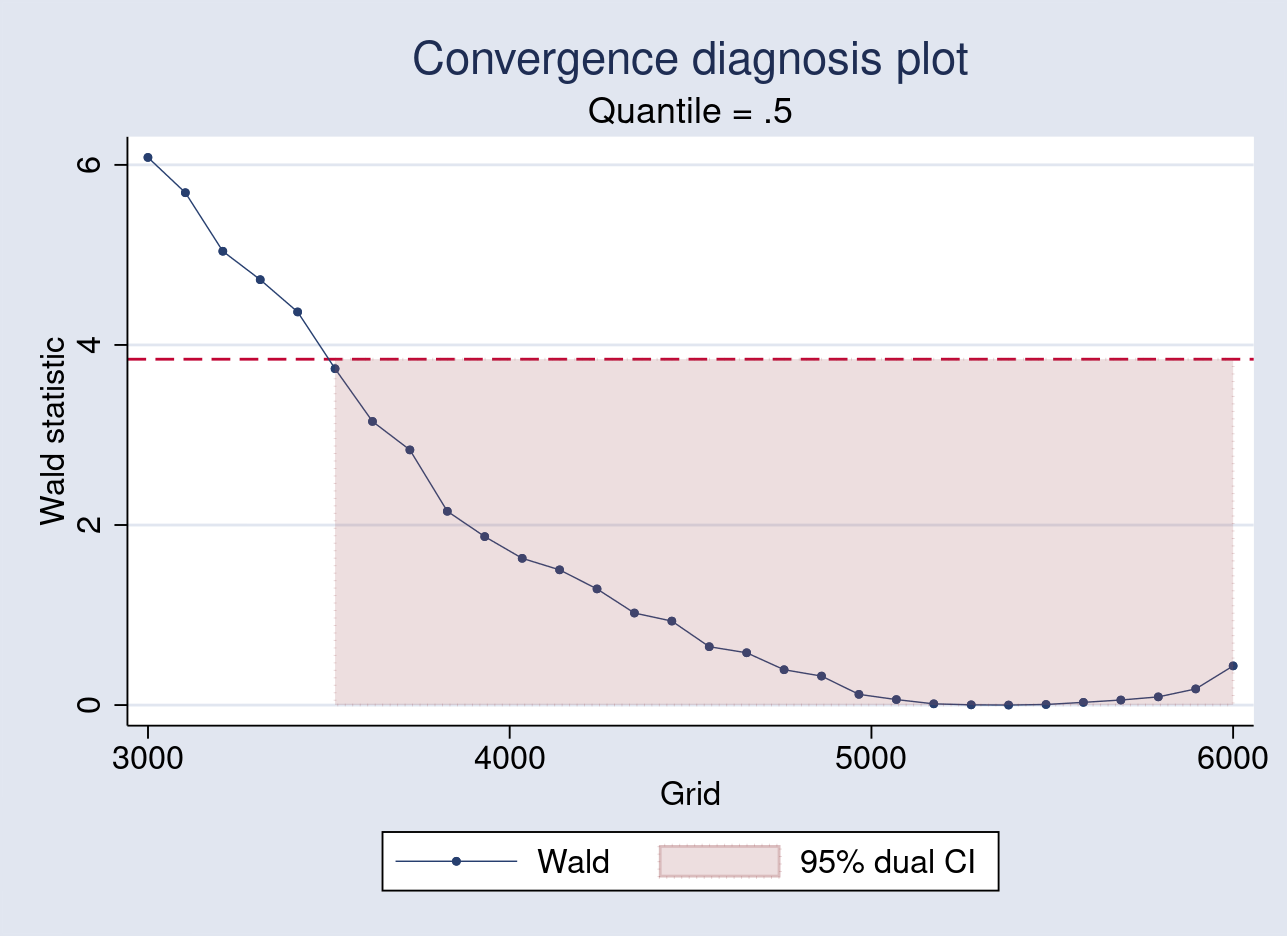
\includegraphics[scale=0.25]{eps/ex4_waldplot2}
\end{figure}

The graph shows that the upper bound $6000$ is too small because we need the
Wald statistics to intersect with the 95\% critical value at both the lower and
upper bound. Now, we can increase the upper bound and see if the IQR estimator
converges. For example, we increase the upper bound to $8000$.

\begin{stlog}
. cap noi ivqregress iqr assets (i.p401k = i.e401k) income age familysize  ///
>         i.married i.ira i.pension i.ownhome educ, bound(3000 8000)
{\smallskip}
Initial grid
    quantile = 0.50: .........10.........20.........30
{\smallskip}
Adaptive grid
    quantile = 0.50: .........10.........20.........30
{\smallskip}
IV median regression                                   Number of obs =   9,913
Estimator: Inverse quantile regression                 Wald chi2(9)  = 1290.41
                                                       Prob > chi2   =  0.0000
{\smallskip}
\HLI{13}{\TOPT}\HLI{64}
             {\VBAR}               Robust
      assets {\VBAR} Coefficient  std. err.      z    P>|z|     [95\% conf. interval]
\HLI{13}{\PLUS}\HLI{64}
     1.p401k {\VBAR}   5332.937   574.5175     9.28   0.000     4206.903    6458.971
      income {\VBAR}    .157381    .012478    12.61   0.000     .1329246    .1818374
         age {\VBAR}   99.78981   8.553978    11.67   0.000     83.02432    116.5553
  familysize {\VBAR}  -199.6165    54.3519    -3.67   0.000    -306.1442   -93.08872
             {\VBAR}
     married {\VBAR}
    Married  {\VBAR}  -1351.309   227.0824    -5.95   0.000    -1796.382   -906.2357
             {\VBAR}
         ira {\VBAR}
        Yes  {\VBAR}   22631.85   1022.023    22.14   0.000     20628.72    24634.98
             {\VBAR}
     pension {\VBAR}
Receives ..  {\VBAR}  -694.1447    210.533    -3.30   0.001    -1106.782   -281.5077
             {\VBAR}
     ownhome {\VBAR}
        Yes  {\VBAR}  -30.67158   154.6947    -0.20   0.843    -333.8676    272.5244
        educ {\VBAR}  -96.30363    32.0715    -3.00   0.003    -159.1626   -33.44465
       _cons {\VBAR}  -4983.758   569.4043    -8.75   0.000     -6099.77   -3867.746
\HLI{13}{\BOTT}\HLI{64}
Endogenous: 0b.p401k 1.p401k
 Exogenous: income age familysize 0b.married 1.married 0b.ira 1.ira
            0b.pension 1.pension 0b.ownhome 1.ownhome educ 0b.e401k 1.e401k
{\smallskip}

\end{stlog}

Now, the IQR estimator converges. We can redraw the Wald plot to confirm that
the proposed grid points interval is indeed wider than the dual confidence
interval.

\begin{stlog}
. estat waldplot, name(c)

\end{stlog}

\begin{figure}[H]
\centering
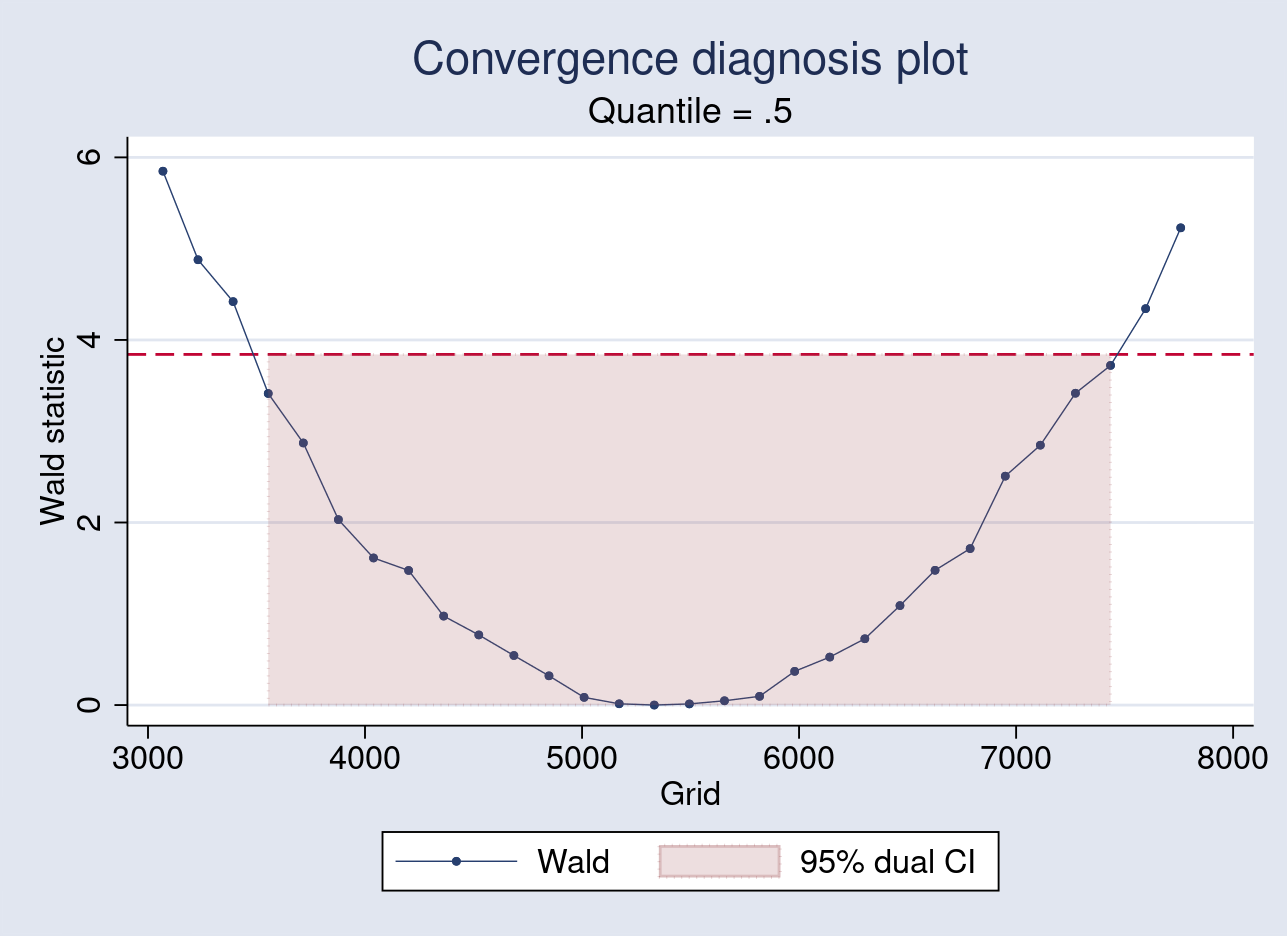
\includegraphics[scale=0.25]{eps/ex4_waldplot3}
\end{figure}
